\documentclass[12pt,a4paper]{report}

\usepackage[utf8]{inputenc}
\usepackage[T1]{fontenc}
\usepackage{lmodern}
\usepackage{titlesec} 
\usepackage{graphicx}
\usepackage{microtype}
\usepackage{hyperref} 
\usepackage[frenchb]{babel}

\usepackage{pict2e}

\usepackage{listings}	  

\lstdefinestyle{customstyle}{
    basicstyle=\footnotesize,
    breakatwhitespace=false,         
    breaklines=true,                 
    captionpos=b,                    
    keepspaces=true,                                                                                       
    tabsize=4,
    frame=single,
    moredelim=[is][\underbar]{_}{_}
}
\lstset{style=customstyle}

\title{Projet de recherche}
\author{Antoine Forgerou \and Jérémy Bardon \and Nicolas Bourdin}
\date{}
\titleformat{\chapter}[hang]{\bf\huge}{\thechapter}{2pc}{} %Permet de masquer les affichages de "Chapitre" 
\begin{document}
	\renewcommand{\contentsname}{Sommaire}
	\maketitle	

	\tableofcontents	
	\newpage
	
	\setlength{\unitlength}{1cm}

\chapter{Présentation du laboratoire}
Acteur central du développement de l'informatique dans la région des Pays de La Loire, le LINA (Laboratoire d'Informatique de Nantes Atlantique) est un laboratoire de recherche en sciences et technologies du logiciel dirigé par Pierre Cointe. %Avec ses 180 membres, celui ci couvre 

\section{Les différentes équipes}
Le LINA est composé des équipes suivantes : 
\begin{itemize}
  \item AeLoS : \textbf{A}rchitecture et \textbf{Lo}giciel \textbf{S}ûrs
  \item ASCOLA : \textbf{AS}pect and \textbf{CO}mposition \textbf{LA}nguages
  \item AtlanMod : \textbf{Atlan}tic \textbf{Mod}eling 
  \item COD : \textbf{CO}nnaissances et \textbf{D}écision
  \item ComBi : \textbf{Com}binatoire et \textbf{Bi}oinformatique
  \item DUKe : \textbf{D}ata \textbf{U}ser \textbf{K}nowledg\textbf{e}
  \item GDD : \textbf{G}estion de \textbf{D}onnées \textbf{D}istribuées
  \item GRIM : \textbf{G}estion, \textbf{R}ésumé, \textbf{I}nterrogation, et apprentissage sur les \textbf{M}asses de données
  \item OPTI : Optimisation globale, optimisation multi-objectifs
  \item TALN : \textbf{T}raitement \textbf{A}utomatique du \textbf{L}angage \textbf{N}aturel
  \item TASC : Programmation par contraintes
\end{itemize}

\chapter{L'équipe AeLoS}	

\chapter{Présentation du sujet}
\section{Problématiques}

\section{Solutions proposées par l'équipe AeLoS}
Pour répondre à la problématique, l'équipe AeLoS nous a proposé 3 façons de 
faire tout en nous laissant la liberté d'en proposer d'autres.
\\\\
Dans le but de simplifier les exemples, nous avons fait le choix de représenter 
les modèles comme des formes géométriques que l'on essayerai d'emboiter.
\\\\
La première solution consiste à adapter un des modèles au deuxième quand cela 
est possible. On peut prendre l'exemple du théorème de Kleene qui assure qu'un 
automate à états finis peut être écrit sous la forme d'une expression 
rationnelle et vice et versa.

\begin{figure}[h]
	\centering
	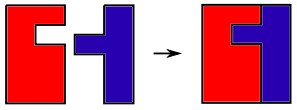
\includegraphics[scale=1]{ressources/solution1.png}
	\caption{Solution 1 - Adaptation d'un modèle}
\end{figure}
\newpage
L'approche qui parait la plus évidente mais qui peut se révéler complexe 
consiste à intégrer un troisième modèle dans le système. Ce dernier va alors 
jouer le rôle de passerelle entre les deux modèles que l'on veut faire 
communiquer.

\begin{figure}[h]
	\centering
	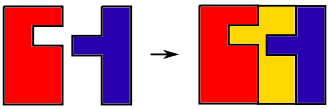
\includegraphics[scale=1]{ressources/solution2.png}
	\caption{Solution 2 - Interface entre les modèles}
\end{figure}

Plug'N'Check est le nom de la troisième solution que l'équipe nous a soumise. 
Le principe est de faire interagir les modèles ensemble puis d'effectuer des 
vérifications pour déterminer si les modèles peuvent communiquer à 100\%, 
en partie ou pas du tout.

\begin{figure}[h]
	\centering
	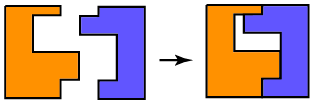
\includegraphics[scale=1]{ressources/solution3.png}
	\caption{Solution 3 - Plug'N'Check}
\end{figure}

Dans le cadre de notre stage d'initiation à la recherche, nous nous sommes 
orientés vers la première solution. Nous avons donc entrepris de transformer 
n'importe quel modèle dans un language commun afin de permettre de les 
interfacer.

\chapter{PDF de présentation du projet}
Contexte : Approches formelle des systèmes embarqués communiquants.
La construction rigoureuse d'un logiciel se fait à partir de son modèle. Pour des logiciels complexes (par exemple ceux
qui ont de nombreux composants différents -- hétérogènes-- et qui communiquent), on a affaire à plusieurs modèles
(hétérogènes aussi) qui doivent intérargir de façon cohérente, pour garantir l'interopérabilité sémantique entre les
modèles puis les composants logiciels. Le domaine des systèmes embarqués (et aussi des objets connectés) regorge
d'exemples.
Description du travail : Etudier l'interopérabilité entre des modèles de composants (logiciels ou non).
En nous appuyant dans un premier temps sur des modèles à base d'automates à états, il s'agit dans le cadre du stage
d'initiation à la recherche, de contribuer à la conception et au développement d'outils passerelle entre modèles.
Nous travaillons sur plusieurs aspects :
- Lorsque cela est possible, en fonction de la sémantique des modèles, un modèle donné est encodé par un autre
modèle choisi mais qui est sémantiquement équivalent.
- Lorsque cela est possible, en fonction de la sémantique des modèles, un modèle peut interagir avec un autre avec
des contrats (de type Assume/Guarantee)
- Plug'N'Check (analyse systématique de modèles/composants)
- etc

\end{document}
